\documentclass{standalone}
\usepackage{tikz}
\usetikzlibrary{intersections, calc}

\begin{document}
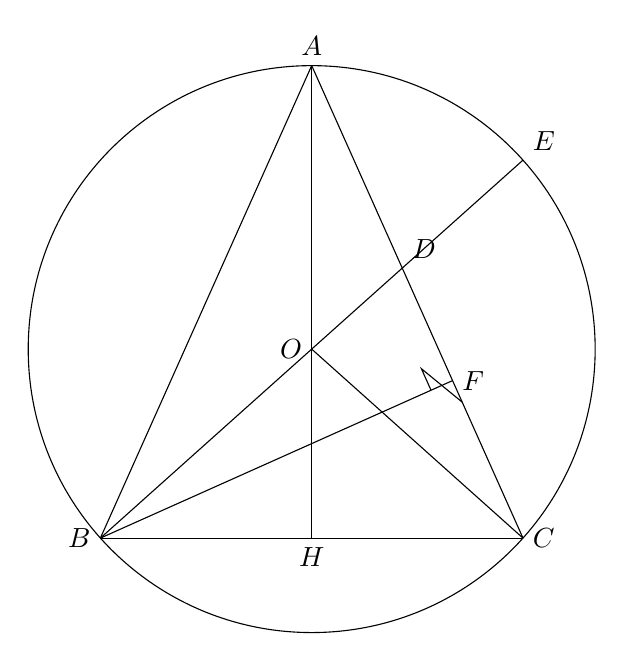
\begin{tikzpicture}[scale=1.2]
    % Define coordinates
    \coordinate (O) at (0,0);
    \coordinate (A) at (0,3);
    \coordinate (H) at (0,-2);
    % B and C on y = -2, circle radius 3
    % x^2 + 4 = 9 => x = sqrt(5) approx 2.236
    \coordinate (B) at (-2.236, -2);
    \coordinate (C) at (2.236, -2);
    % E is opposite B
    \coordinate (E) at (2.236, 2);

    % Circle
    \draw (O) circle (3);

    % Paths for intersection
    \path [name path=AC] (A) -- (C);
    \path [name path=BE] (B) -- (E);

    % Intersection D
    \path [name intersections={of=AC and BE, by=D}];

    % Point F (projection of B onto AC)
    \coordinate (F) at ($(A)!(B)!(C)$);

    % Drawing lines
    % Triangle ABC
    \draw (A) -- (B);
    \draw (A) -- (C);
    \draw (B) -- (C);
    
    % Diameter BE
    \draw (B) -- (E);
    
    % Vertical line AH
    % Instruction: AO is solid (changed from dashed). OH is solid.
    \draw (A) -- (O);
    \draw (O) -- (H);
    
    % Radius OC
    \draw (O) -- (C);
    
    % Altitude BF
    \draw (B) -- (F);
    
    % Right angle at F
    \draw ($(F)!2.5mm!(B)$) -- ($(F)!2.5mm!(B)!1!90:(F)$) -- ($(F)!2.5mm!(C)$);

    % Labels
    \node[above] at (A) {$A$};
    \node[left] at (B) {$B$};
    \node[right] at (C) {$C$};
    \node[left] at (O) {$O$};
    \node[below] at (H) {$H$};
    \node[above right] at (E) {$E$};
    \node[above right] at (D) {$D$};
    \node[right] at (F) {$F$};
\end{tikzpicture}
\end{document}
